\documentclass[a4paper,11pt]{article}
\usepackage[style=numeric,natbib=true,sorting=none,maxbibnames=99]{biblatex}
\usepackage{enumitem}
\usepackage{hyperref}
\usepackage{float}
\usepackage{url}
\usepackage{graphicx}
\graphicspath{ {./img/} }
\usepackage{subcaption}
\captionsetup{compatibility=false}
\bibliography{references.bib}

\begin{document}
\title{Analyzing Tor Artifacts in Memory \\~\\
\large{Cyber Crime and Forensics \\
Master Security and Network Engineering\\  University of Amsterdam\\
Project report\\}
\textbf{Version:} 1.0}
\author{
    Axel Koolhaas \texttt{a.e.koolhaas@student.vu.nl} \and
    Alexandros Dimos \texttt{a.dimos@student.vu.nl}\\
    \\
}
\date{
    \textnormal \today
}
\maketitle

\clearpage

\section*{Abstract}

\textbf{Keywords: }
\clearpage

\tableofcontents
\clearpage

\section{Introduction}
\label{sec:introduction}


For this purpose, we define the following research question:
\textit{Question}
We have the following sub questions:
\begin{enumerate}
    \item sub 1
    \item sub 2
\end{enumerate}

\section{Related work}
\label{sec:related_work}

There has been some previous work on web browser artifacts. One
research proved that it was possible to reconstruct video content
played in Chrome browser by using locally buffered cache data on
the hard drive. \cite{horsman2018reconstructing}

Horsman also tried to prove if somebody viewed an image bases on the
hard drive cache files of both Mozilla Firefox and Google
Chrome. However, testing highlighted inconsistent cache behaviour,
meaning that it may not possible to make an accurate assumption of
which images were viewed by a user based on cached content alone.
\cite{horsman2018didn}

Another interesting research was done on artifacts left behind by
private browser modes. All large web browsers were researched,
e.g. Chrome, Firefox and Safari. The majority of important artifacts
with regard to privacy are removed by the browsers, but users did not
take into account the impact of artifacts with low or medium valuation
being left behind \cite{tsalis2017exploring}. One of mitigations
presented in this paper is storing data into the RAM. This decreases
the chance of confidential data leaks. However, as we present in our
paper, forensic experts can still extract artifacts from RAM,
disproving the mitigation. Also, these three papers use cache located
on the hard drive for finding artifacts.

A paper which resembles our technique, i.e. recovering artifacts from
RAM, is the research done by Yang et al, where they managed to recover
login credentials from private browsing sessions from RAM
\cite{yang2017applying}. This paper is interesting from a technical
perspective, but not so much from a forensic perspective.

The most important related work is the work done by a previous
Cybercrime and Forensics group in 2018. They managed to reconstruct
the entire GUI of a Chromium-based browser from a memory image
\cite{wikner2018reconstruct}. Their work is very interesting, but
unfortunately not suited for this project because it is focused on a
different browser with different datastructures.

\section{Methods}
\label{sec:methods}


\section{Implementation}
\label{sec:implementation}

In this section we will describe the implementation of our approach,
as well as the techniques used to recover the DOM tree. The first step
in our method is to reverse engineer the low level Mozilla Firefox
data structures. This will hopefully give us insight in the browser's
internals and will help us find a way to traverse the DOM tree.

\subsection{Important Classes}
First, we need to find the some structures that are used as DOM
nodes. Browsing through the source of Firefox with Mozilla
DXR\cite{dxrmozilla} we found the
nsINode\footnote{\url{https://dxr.mozilla.org/mozilla-esr60/source/dom/base/nsINode.h}}
class that serves as base for the higher level objects and implements
some basic functionality of a tree. Every
HTMLElement\footnote{\url{https://dxr.mozilla.org/mozilla-esr60/source/dom/html/nsGenericHTMLElement.h}}
object inherits from nsINode. It contains a doubly linked list via
\textit{mNextSibling} and \textit{mPreviousSibling} to identify
objects on the same tree level. Here we can also find
\textit{mParent}, a reference to the parent element in the DOM and
\textit{mFirstChild}, a reference to the first child. We can use these
4 pointers in order to traverse the whole DOM. However we are missing
one key component: the root node.

In Firefox, the root of the tree is the
DocumentElement\footnote{\url{https://dxr.mozilla.org/mozilla-esr60/source/dom/html/nsHTMLDocument.h}}. This
class contains a lot of metadata such as: URL, referrer,
last\_focus\_time, links to objects for CSS style sheets, etc. The
amount of information in this class is enormous and we did not manage
to understand even half of the fields. However we know it is the
starting point of the DOM so it suffices to find this object in memory
and then we can traverse the whole tree with the four pointers
previously mentioned.

\subsection{Reverse Engineering}
Before we try to automate any information extraction from memory
dumps, we first need to understand the layout of the above mentioned
classes in memory. Unfortunately, the source code does not provide
reliable information because, during compilation time, fields might
get rearranged or merged for performance reasons. Compiler
optimizations also make the memory layout of an object sometimes very
hard to understand. Thus, we opted to reverse engineer the memory
objects using GDB to perform dynamic analysis.  In order to make this
reverse engineering process easier, we will use the debug symbols that
we have for out tor compilation as we explained in
section~\ref{sec:methods}. The first problem that we encounter is
introduced by the huge and randomized 64 bit address space. We know we
are looking for nsINode objects in memory but we do not know where to
find them. Our approach to identifying such memory locations is to use
debugger breakpoints in the constructors of the classes of interest
(in this case nsINode). The whole technique goes as follows:
\begin{enumerate}
\item We run the browser but without going to any page.
\item We attach to the browser process with GDB.
\item We place a break point in the class constructor for which we want
  to find an object.
\item We \textbf{continue} execution in GDB.
\item We type the URL of a page and instruct the browser to fetch it.
\item At this point the browser stops in the break point previously
  placed since it tries to create DOM objects. We look at GDB and
  note down the address of the \textit{this} parameter of the
  constructor. The variable \textit{this} is not explicitly typed in
  C++ but the compiler implicitly uses it. It refers to the address of
  the object.
\item We detach from the browser process. We explain later why.
\item We re-attach to the browser process and use the memory location
  previously retrieved as well as the debug symbols to read
  memory. This is as straightforward as casting the memory location to
  the object of the desired type (nsINode).
\item Now we can clearly see the whole object with every field name,
  but most importantly with every value at this particular point in
  time.
\end{enumerate}

We can use this technique to find any object. However, we are
interested in a few specific objects: nsINode and its
descendants. Later we apply the same technique to recover the
DocumentElement\footnote{\url{https://dxr.mozilla.org/mozilla-esr60/source/dom/html/nsHTMLDocument.h}}.

We need to detach from the process on step 7 because repeated
errors occur. As we explained in a previous section Firefox uses more
than one processes. Notably, it uses one process for the GUI and one
process for each tab open. This means that the GUI and the tab
processes have to communicate between them. When we attach to the tab
process we do not take into account this communication between the
processes. Blocking the tab process disrupts this communication which
in turn makes both processes enter different error treating
routines. These routines usually involve signal throwing and
handling. GDB, by default, catches all signals sent to the process and
while this behavior can be disabled, it has to be done for each and
every signal. This can also cause malfunctioning of GDB in a later
stage. To avoid these problems, we opted to detach from the
process, let it run all of its error recovering routines, and then
re-attach when the process is in a robust state.

\subsection{Locating the DocumentElement}
As we saw earlier, in order to recover the DOM tree we need to start
from the DocumentElement. This element stands as root of the
tree. Whilst reverse engineering, we had the luxury of placing
breakpoints in the constructor to find this element. But our actual
goal is to be able to locate it in a memory dump of the tab
process. To achieve this we introduce a second technique that relies
on string search, pointer search and a better understanding on how
element types are stored in Firefox.

Each element contains a pointer to a
NodeInfo\footnote{\url{https://dxr.mozilla.org/mozilla-esr60/source/dom/base/NodeInfo.h}}
object. This is an optimization that the Firefox developers implement
to save some memory space. All information regarding an element type
("HTML", "body", "head", "div", etc) is stored in a NodeInfo
object. Then all elements of that type keep a reference to that. As an
example all divs point to the same div NodeInfo object. This object is
very important because it contains a pointer to the document of origin
since different documents may have different types. The
DocumentElement has a NodeInfo of type "\#document". Two other
interesting NodeInfo objects are the "\#text" NodeInfo, which
represent all leaf nodes that contain text and the "\#comment"
Nodeinfo, which contains all comments (in Firefox comments are part of
the DOM tree).

Our approach will focus on locating the "\#document" NodeInfo object
and from there finding the reference to the DocumentElement. Field
specific information such as pointers in an object are found by using
their corresponding offset from the object start. We learn these
offsets whilst reverse engineering and they are fixed. However, the
downside is that different versions of the source code may lead to
different offsets of these fields in memory. In essence the technique
is the same but the offsets may vary from version to version. We
divided the technique into the following steps:

\begin{enumerate}
\item We perform a search for the string "\#document" with null bytes
  in-between each letter. The null bytes appear because Firefox
  developers decided to use 16 bit char strings instead of 8. This
  search yields multiple results.
\item For each string we pack its address to the corresponding
  endianness (little endian for our Ubuntu machine) and once again
  perform a search in the whole dump. With this search we aim to find
  pointers towards the string "\#document". These pointers could be
  part of the NodeInfo object for "\#document". Again multiple results
  are yielded.
\item We perform a sanity check to make sure that the pointer is part
  of a NodeInfo object. Specifically, we look at the first field of
  the alleged object which should be the \textit{mRefcount} field. In
  this field the number of objects referencing this object is stored
  for efficient memory management. During our reverse engineering we
  found this value to be higher than 0 and lower than 10. Nonetheless,
  we check if it is lower than 100. In case the object under
  inspection is not a NodeInfo object, this value will be either a
  pointer which is a very big value (ex: 0x7fffff8070) or 0. This
  check eliminates a lot of the false positives.
\item For each result that passed the sanity check, we read the
  \textit{mDocument} field. We decode the pointer which is the
  starting point of a Document Element. However, in Firefox there are
  multiple types of documents but we are interested only in
  "HTMLDocument"s. For that reason, we perform a second sanity check at
  this point. In the vtable of the DocumentElement object, a pointer to
  a string can be found with the name of the document type. We read
  that pointer and its contents; we stop if it is not "HTMLDocument".
\item We end up with a list of pointers to HTMLDocument elements and
  when removing duplicates only 1 element remains. This happens
  because in Firefox new HTML documents are opened in new tabs and
  thus in new processes.
\end{enumerate}

This procedure takes approximately 20 seconds for a dump of 1.7 GB
which is not uncommon considering that the dump contains all the
shared libraries also. Once the DocumentElement is found in memory, we
can start reading its fields to start information acquisition. Since
we did not manage to reverse engineer the whole structure, we limit
ourselves to reading just the OriginalURI and DocumentURI fields that
represent the URL and the referrer field.

\subsection{Traversing the DOM tree}
We perform the traversal of the tree in a depth first manner starting
from the DocumentElement. We read children first and then siblings. In
contrast with the previous operation, this takes seconds to perform
since we are not scanning memory but reading from already known
offsets continuously. At the end we have an internal representation of
the tree in our program, that contains the address of each node, its
type and its link pointers (siblings, parent, child). We can search,
print, or perform other operations at our leisure.

\subsection{Reading text and comment nodes}
In Firefox, depending on the type of element (and simultaneously of
the type of NodeInfo), the element object may contain a different
field. One of those situational fields is the \textit{mText} which
appears only in text and comment nodes. The type of this field is a
Mozilla internal string structure which contains the bytes and the
length of the string. As soon as we detect a text or comment node (by
reading its NodeInfo structure), we also parse the \textit{mText}
field. Thus, we recover all the text and comments from the DOM.

\subsection{Recovering links, images and videos}
While we do not manage to recover individual attributes, some of them
are accessible to us. Links, images, videos, and possibly other
elements that we did not reverse engineer store important metadata as
situational fields like \textit{mText} for text nodes. This means that
even if links, images and videos have their sources in the attributes,
we can still find them by parsing the object. In this particular case
there are fields that hold the sources for links (\textit{mURI}),
images(\textit{mLastSelectedSrc}), and videos(\textit{mLoadSrc}). We
read these fields and extract the URLs for these 3 common types of
elements.

\subsection{Putting it together}
Using the above information, we recreate the HTML in a rudimentary
fashion using a Python script. The text recovery works always and is
100\% accurate. Unfortunately, only a small part of what the user sees
is the text and even then, the CSS styling and HTML attributes might
change an element's appearance completely. We present some of the
recreated HTML in section~\ref{sec:results}.

\section{Results}
\label{sec:results}

Following the implementation details presented in the previous section
we created a tool that automatically, given a dump of a Tor/Firefox
tab, will find the DocumentElement. Afterwards, it will extract the
DOM nodes while checking their type. For the text and comment nodes,
the tool will read the \textit{mText} field while for "a", "img" and
"video" nodes it reads the corresponding source fields described in
the previous section. The output of the tool consists of: URL of the
current tab, referrer of the current tab and the incomplete
reconstructed HTML which is put in the "./dump.html" file. The created
HTML has the same text nodes but the structure of the tree often is
different. This happens because there are nodes in the DOM that are
not shown in the browser inspector. These nodes are not part of the
HTML, they are added by the browser for various reasons that we do not
fully know. In this section, we show how we run the tool and what
output we get for 3 websites: os3.nl\cite{os3nl}, ccf website (clicked
on the CCF link)\cite{os3ccfnl} and
http://zqktlwi4fecvo6ri.onion/wiki/index.php/Main\_Page which is the
full version of the hidden wiki\cite{thehiddenwiki}.

\subsection{Usage}
The tool is written in Python and takes as parameter the directory
containing the dumped Tor virtual address space. A directory is needed
due to the way that Volatility extracts the address space: each
virtual mapping is put in a separate file. This dump is extracted in
advance using Volatility's \textbf{linux\_dump\_map (dump\_map for
  windows)} command.

\subsection{Simple Website}
As a simple test, we typed \textbf{os3.nl} in the URL bar and hit
enter. When we run the tool, we get the output in
figure~\ref{img:output1}. We can see the correct URL return and the
null referrer field (since the URL was typed).

\begin{figure}[h]
  \centering 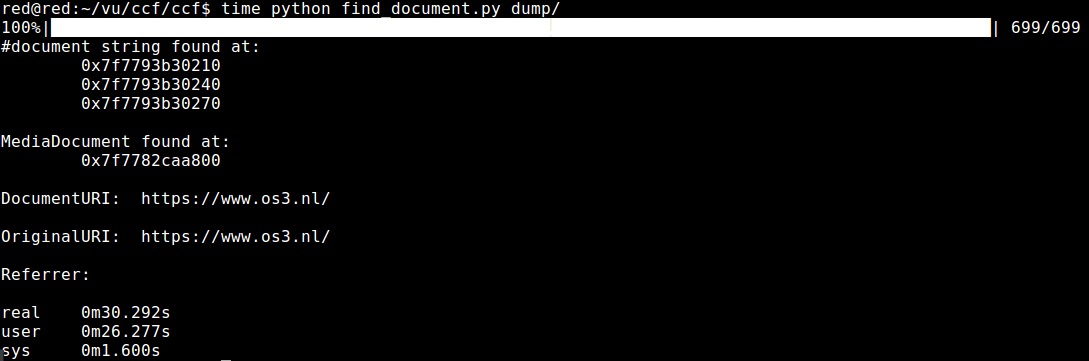
\includegraphics[scale=0.35]{output1}
  \caption{Output when running the tool on the dump generated for the
    os3.nl visit.}
  \label{img:output1}
\end{figure}

When we look at the HTML produced, we can see that the text is the
same but the lack of styling and attributes makes the pages look very
different. A small comparison can be seen in
figure~\ref{fig:os3_compare}. This HTML mismatch is expected and can
be improved with future work on attributes and CSS styles. However,
content can arguably be deduced during an investigation, even from
incomplete recreated HTML.

\begin{figure}[h]
  \begin{subfigure}{\linewidth} \centering
    
\includegraphics[scale=0.35]{os3_orig1}
    \caption{Original os3.nl website.}
  \end{subfigure}\\[1ex]

  \begin{subfigure}{\linewidth} \centering
    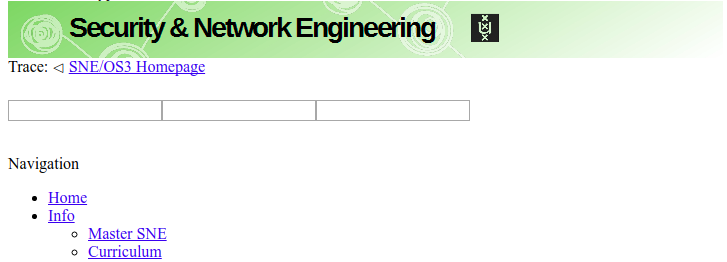
\includegraphics[scale=0.35]{os3_recovered1}
    \caption{Reconstructed HTML from os3.nl website.}
  \end{subfigure}
  \caption{Comparison between original and reconstructed os3.nl HTML.}
  \label{fig:os3_compare}
\end{figure}

\subsection{Referrer}
In order to check the referrer field, we clicked on the "CCF" link of
the previously browsed website. The result, as seen in
figure~\ref{img:output2} is correct: the referrer points to the os3.nl
website where we clicked the link. The recovered HTML again contains
true text but completely wrong styling, although some elements, such
as tables, maintain a good aspect even without styling as seen in
figure~\ref{fig:ccf_compare}.

\begin{figure}[h] \centering 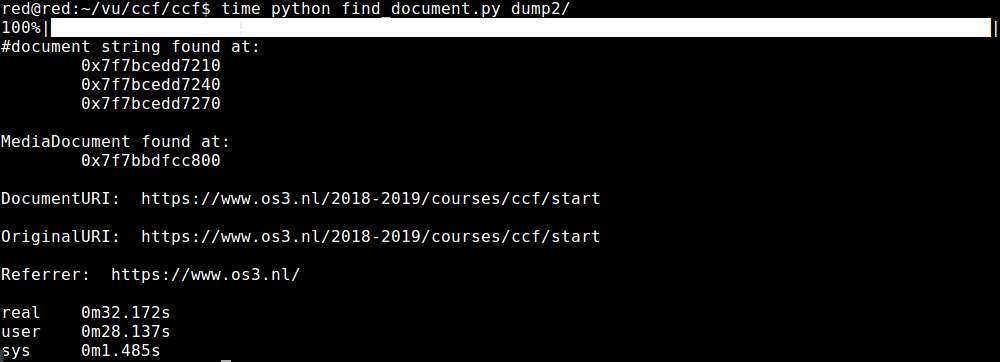
\includegraphics[scale=0.35]{output2}
  \caption{Output when running the tool on the dump generated for the
    CCF link click.}
  \label{img:output2}
\end{figure}

\begin{figure}[h]
  \begin{subfigure}{\linewidth} \centering
    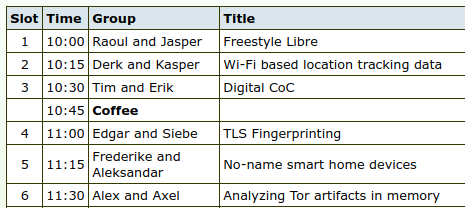
\includegraphics[scale=0.35]{ccf_orig1}
    \caption{Original ccf website.}
  \end{subfigure}\\[1ex]

  \begin{subfigure}{\linewidth} \centering
    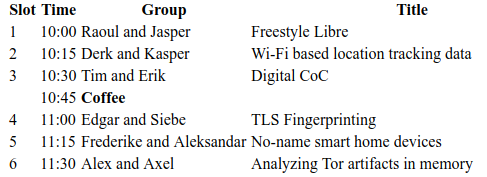
\includegraphics[scale=0.35]{ccf_recovered}
    \caption{Reconstructed HTML from ccf website.}
  \end{subfigure}
  \caption{Comparison between original and reconstructed ccf HTML.}
  \label{fig:ccf_compare}
\end{figure}

\subsection{Onion Website}
We also tried the tool on a \textit{.onion} website. Our expectation
was that the tool will work the same since the same exact memory
structures are used to represent the DOMs for \textit{.onion}
websites. As can be seen in figures~\ref{img:output3}
and~\ref{fig:hidden_compare} the results are similar to normal
webpages. An important observation is that for \textit{.onion}
websites, opening the reconstructed HTML with a default browser will
not show any images due to their origin being behind a \textit{.onion}
URL. The tool still recovers the correct source as can be seen
in~\ref{img:onion_img}.

\begin{figure}[h]
  \centering 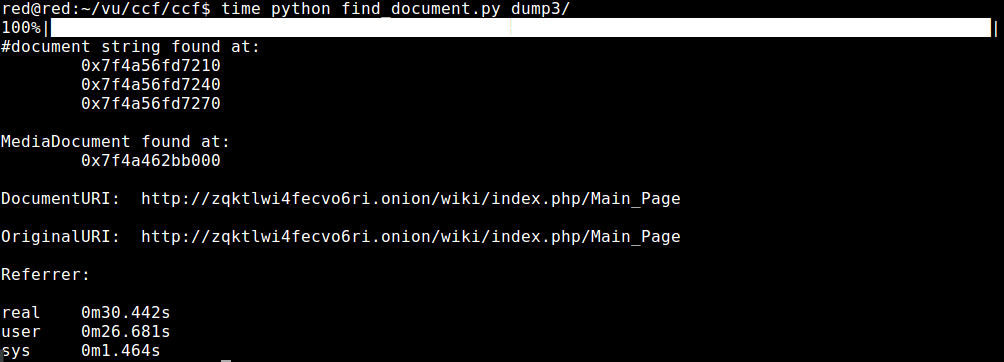
\includegraphics[scale=0.35]{output3}
  \caption{Output when running the tool on the dump generated for the
    hidden wiki \textit{.onion} website.}
  \label{img:output3}
\end{figure}

\begin{figure}[H]
  \begin{subfigure}{\linewidth}
    \centering 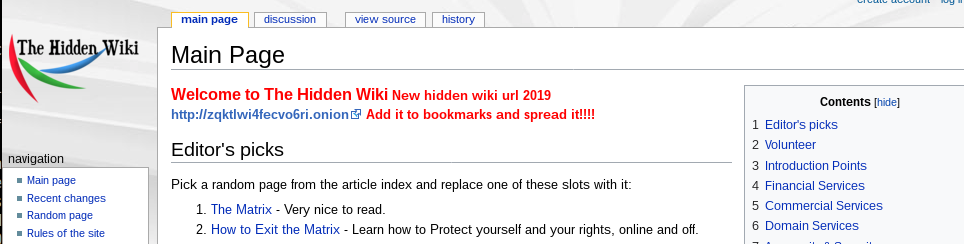
\includegraphics[scale=0.35]{hidden_orig}
    \caption{Original hidden wiki website.}
  \end{subfigure}\\[1ex]

  \begin{subfigure}{\linewidth}
    \centering 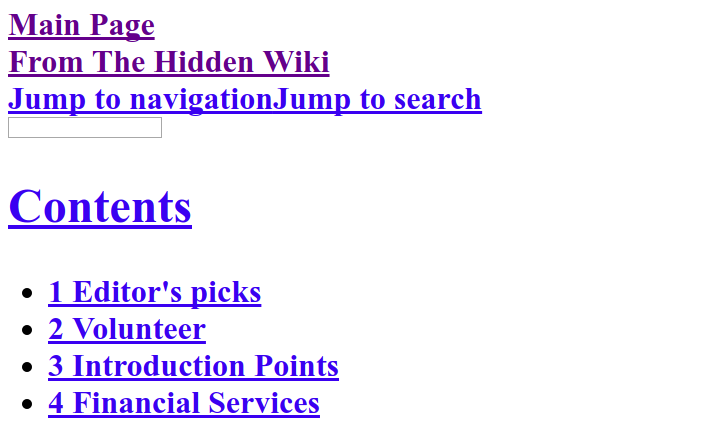
\includegraphics[scale=0.35]{hidden_recovered}
    \caption{Reconstructed HTML from hidden wiki website.}
  \end{subfigure}
  \caption{Comparison between original and reconstructed hidden wiki
    HTML.}
  \label{fig:hidden_compare}
\end{figure}

\begin{figure}[H]
  \centering 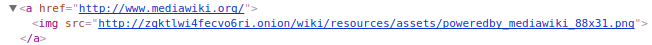
\includegraphics[scale=0.65]{onion_img}
  \caption{img element reconstructed with correct src.}
  \label{img:onion_img}
\end{figure}

\subsection{Run time}
In all of the test cases we run the tool under the unix \textbf{time}
command to see the exact durations of the execution. We show that for
dumps of 1.7GB the tool take approximately 30 seconds to recover the
data, where the biggest part is spent finding the
DocumentElement. This demonstrates that the approach is quite fast and
can parse through big HTML documents in matters of minutes.

\section{Discussion}
\label{sec:discussion}
\section{Conclusion}
\label{sec:conclusion}
\printbibliography

\end{document}
